\documentclass[11pt,a4paper,oneside]{report}

\usepackage{graphicx} % Enhanced support for graphics
\usepackage{booktabs} % \toprule, \midrule, \bottomrule for clean tables
\graphicspath{ {./images/} }

\usepackage[tmargin=1in,bmargin=1in,lmargin=1.38in,rmargin=0.79in]{geometry} % Surrey Normal margins

\usepackage{times} % Adobe Times Roman (or equivalent) as default font
\usepackage{epsfig} % Include Encapsulated PostScript in LaTeX document
\usepackage{fancyhdr} % Extensive control of page headers and footers
\usepackage{longtable} % Allow tables to flow over page boundaries
\usepackage{subfig} % Manipulation and reference of small subfigures
\usepackage{color} % Colour control
\usepackage{amsmath} % Mathematical typesetting
\usepackage{amssymb} % Extended symbol collection
\usepackage{bm} % Bold symbols in maths mode
\usepackage{psfrag} % Proper math symbols in postscript plots
\usepackage{url} % Allow URLs to be entered
\usepackage[linktocpage]{hyperref} % Extensive support for hypertext

\usepackage[square,numbers]{natbib} % Bibliography

\definecolor{ashgrey}{rgb}{0.7, 0.75, 0.71}

\usepackage{setspace} % Custom line spacing
\usepackage{multicol} % Intermix single and multiple columns
\usepackage{paralist} % Enumerate and itemize within paragraphs
\usepackage{floatrow} % Modifying the layout of floats

\setlength{\parskip}{\baselineskip} % Force skip line between paragraphs
\floatsetup[table]{capposition=top} % Position caption on top of tables

%%% Surrey chapter/section heading requirements %%%
\usepackage{titlesec}
\titleformat{\chapter}[block]
{\fontsize{12}{15}\bfseries}
{\thechapter}
{1em}
{\MakeUppercase}
\titlespacing*{\chapter}{0pt}{1pt}{0pt}[0pt]

\titleformat{\section}[block]
{\fontsize{12}{15}\bfseries}
{\thesection}
{1em}
{}
\titlespacing*{\section}{0pt}{0pt}{-12pt}[0pt]

\titleformat{\subsection}[block]
{\fontsize{12}{15}\bfseries}
{\thesubsection}
{1em}
{}
\titlespacing*{\subsection}{0pt}{0pt}{-12pt}[0pt]

\titleformat{\subsubsection}[block]
{\fontsize{12}{15}}
{\thesubsubsection}
{1em}
{}
\titlespacing*{\subsubsection}{0pt}{0pt}{-12pt}[0pt]
%%%%%%

\newcommand{\squeezeup}{\vspace{-2.5mm}}
\clubpenalty = 10000
\widowpenalty = 10000

\usepackage{style/myfootnote}
\makesavenoteenv{longtable}
\usepackage{vmargin}
\input{./style/epsf.sty}

\input{./parameters/param}

%%%%%%%%%%%%%%%%%%%%%%%%%%%%%%%%%%%%%%%%%%
\begin{document}
\normalsize
\rhead{\textcolor{ashgrey}{Deepakraj Rajmohan, MSc dissertation --- interim draft}}
\renewcommand{\headrulewidth}{0pt}

%%%%%%%%%%%%%%%%%COVER PAGE%%%%%%%%%%%%%%%%%
\begin{center}
{\LARGE {\vspace*{0.5cm}\Huge\bf Generative Modelling for Realistic Mars Landing Site Visualisation}}

\vspace{2em}
{\large\textit{Interim Draft }}

\vspace{3em}
        {\Large \bf Deepakraj Rajmohan}\\
        \vspace{2em}
        {\Large\textit{Master of Science in Artificial Intelligence}\\
        from the\\
        University of Surrey\\
        \vspace{2em}
        \centering
        
\includegraphics[width=0.6\textwidth]{logo.png}\\
        \vspace{2em}
        \textit{School of Computer Science and Electrical and Electronic Engineering}\\
		 Faculty of Engineering and Physical Sciences\\
		University of Surrey\\
		Guildford, Surrey, GU2 7XH, UK\\
        \vspace{2em}
        September 2026\\
       Supervised by: Dr Xiatian Zhu\\
        \vspace{\stretch{1}}}
        \textcopyright\ Deepakraj Rajmohan 2026
\end{center}
\pagenumbering{roman}

%%%%%%%%%%%%%%%%DECLARATION%%%%%%%%%%%%%%%%%%%%
\clearpage
\newpage
\addcontentsline{toc}{chapter}{Declaration of Originality}
\input{chapters/declaration}

%%%%%%%%%%%%%%%%WORD COUNT%%%%%%%%%%%%%%%%%%%%
\clearpage
\newpage
\addcontentsline{toc}{chapter}{Word Count}
\chapter*{Word Count}

\noindent \textit{This is an interim draft covering the chapters completed to date (Introduction through Results and Diagnosis). A Conclusions chapter has not yet been written, so the counts below will change substantially before final submission.}

\vspace{1em}
\noindent Number of Pages: [to be finalised at submission]

\noindent Number of Words: [to be finalised at submission]


%%%%%%%%%%%%%%%%%%ABSTRACT%%%%%%%%%%%%%%%%%%%
\clearpage
\addcontentsline{toc}{chapter}{Abstract}
\chapter*{Abstract}

Mission planning and astronaut/operator training for planetary exploration increasingly rely on immersive VR reconstructions of candidate landing sites, but the only data available for most such sites is nadir orbital imagery (e.g.\ NASA's HiRISE, 25\,cm/px), not the ground-level, perspective views that make a VR scene feel navigable. This dissertation addresses that nadir-to-perspective domain gap in the context of ESA's ExoMars Rosalind Franklin rover mission, proposing a three-stage generative pipeline --- diffusion-based super-resolution, physics-constrained unpaired view translation, and Gaussian Splatting scene reconstruction --- to turn orbital imagery into explorable, physically plausible VR environments.

To date, the literature review and methodology have been completed, surveying the super-resolution, image-to-image translation, neural rendering, and hallucination-safety literature relevant to each stage, and formalising the proposed Neural Schr\"{o}dinger Bridge formulation, evaluation framework (FID, shadow-angle error, hallucination rate, VR frame rate), and baseline comparisons (MARSGAN, DiffusionSat, CycleGAN, UNSB-no-physics). A CycleGAN baseline for Stage 2 has been implemented, trained, and evaluated end-to-end: a real-resolution HiRISE data pipeline was built after an initial corpus was found to use browse-quality (\textasciitilde3\,m/px) imagery rather than the true 25\,cm/px RDR products, and a corrected \textasciitilde30,000-patch corpus was assembled from seven Oxia Planum observations. A 50-epoch training run on this corrected corpus was completed and evaluated (FID 269.9), and a specific, evidenced diagnosis was reached: one discriminator collapses from epoch 3 onward, most likely because the grainy, true-resolution HiRISE patches hand it an easy non-semantic shortcut over the smoother rover imagery, starving the corresponding generator of a useful gradient. In parallel, a CTX/HiRISE co-registration pipeline for the Stage 1 super-resolution corpus is under development.

This draft covers the work completed to date; addressing the CycleGAN discriminator imbalance, building the physics-constrained UNSB stage, and evaluating the full pipeline remain the subject of ongoing work.


%%%%%%%%%%%%%%%%%%%%TOC%%%%%%%%%%%%%%%%%%%%%
\begin{spacing}{0.1}
	\tableofcontents
\end{spacing}

%%%%%%%%%%%%%%%%%FIGURES%%%%%%%%%%%%%%%%%%%%%
\clearpage
\addcontentsline{toc}{chapter}{List of figures}
\begin{spacing}{1.4}
\listoffigures
\end{spacing}

\newpage
\pagenumbering{arabic}

\pagestyle{fancyplain}
\renewcommand{\headrulewidth}{0pt}
\renewcommand{\footrulewidth}{0pt}

%%%%%%%%%%%%%%%%CHAPTERS COMPLETED TO DATE%%%%%%%%%%%%%%%%%%%%%
\chapter{Introduction}

Planetary exploration missions increasingly depend on immersive virtual-reality (VR) environments for mission planning, hazard assessment, and astronaut or rover-operator training. Building a convincing VR reconstruction of a Mars landing site, however, runs into a basic data problem: the only imagery available for almost every candidate site, including all ExoMars candidate landing areas, is nadir orbital imagery captured from orbit looking straight down, whereas a usable VR scene needs ground-level, perspective imagery of the kind a rover's own cameras produce after it has landed. This dissertation is concerned with closing that nadir-to-perspective domain gap using generative modelling, so that orbital data alone --- available years before any rover touches down --- can be turned into a physically plausible, explorable VR surface.

The work is computational and experimental in nature: it combines remote-sensing data engineering (acquiring and correctly processing real orbital and rover imagery), generative model design and training (image-to-image translation and super-resolution networks), and, in later stages, real-time neural rendering. The concrete application context is ESA's ExoMars Rosalind Franklin rover mission, and the primary test site is Oxia Planum, the mission's selected landing area.

\section{Background and Context}

High-resolution orbital imagery of Mars is comparatively abundant: NASA's HiRISE instrument has imaged large fractions of the surface at up to 25\,cm/pixel, resolving individual boulders and small craters. This is nadir imagery --- captured looking straight down from orbit --- and it is systematically unlike the perspective, oblique, ground-level imagery captured by rover cameras such as NAVCAM, which show terrain from roughly a metre above the surface, with strong foreshortening, occlusion, and local lighting effects that a top-down orbital image simply does not contain. No dataset of geographically \emph{aligned} nadir/perspective Mars image pairs exists, because rover imagery only exists for the handful of sites a rover has actually visited, and even then the rover was never positioned to recreate an orbital viewing geometry. Any method that aims to synthesise rover-perspective imagery from orbital data must therefore work without paired supervision.

This gap sits at the intersection of several active research areas surveyed in Chapter~2: single-image super-resolution (to recover resolution lost between coarser orbital instruments and HiRISE), unpaired image-to-image translation (CycleGAN-style methods, and more recent physics-informed variants such as the Neural Schr\"{o}dinger Bridge), neural scene rendering (NeRF and Gaussian Splatting for turning a set of synthetic views into an explorable 3D scene), and the emerging concern, specific to generative models used for scientific and mission-critical purposes, of hallucination: a model may produce a plausible-looking rock or crater that was never actually present, which is a materially different failure mode from a blurry or low-fidelity output. Existing single-modality approaches (pure super-resolution, or pure style-transfer GANs) each solve part of this problem but none combines resolution recovery, physically-grounded view translation, and real-time rendering into a single pipeline validated against Mars-specific physical plausibility criteria, which is the gap this dissertation addresses.

\section{Objectives}

The objectives below were carried forward from the initial project proposal and refined during the methodology stage (Chapter~3) once the literature review had established that no existing method closes the nadir-to-rover-perspective gap end-to-end for Mars surface synthesis:

\begin{itemize}
	\item \textbf{O1.} Produce nadir imagery at 25\,cm/pixel from coarser CaSSIS/CTX inputs when HiRISE coverage is absent.
	\item \textbf{O2.} Translate unpaired HiRISE nadir patches into statistically plausible rover-perspective images whose photometric and morphometric properties are consistent with Mars surface physics.
	\item \textbf{O3.} Reconstruct a real-time renderable 3D scene from the synthetic perspective images at VR frame rates ($\geq$\,72\,fps).
	\item \textbf{O4.} Quantify the fidelity and physical plausibility of generated imagery against held-out real rover data and known planetary surface statistics.
\end{itemize}

Work to date has focused on the data engineering and baseline modelling required to make O1 and O2 tractable: building correct, real-resolution training corpora for both the orbital and rover domains, and implementing, training, and rigorously evaluating a CycleGAN baseline for O2 before moving to the physics-constrained architecture the methodology proposes. O3 and O4 remain future work.

\section{Achievements}

To date, the following has been completed:

\begin{itemize}
	\item A full literature review (Chapter~2) covering seven topic clusters --- orbital data constraints, super-resolution, image-to-image translation, digital terrain modelling, neural scene rendering, VR reconstruction, and generative hallucination --- synthesising 20 papers into a comparative analysis that motivates the proposed architecture.
	\item A complete methodology (Chapter~3) formalising the three-stage pipeline, including the Neural Schr\"{o}dinger Bridge formulation with four physics-informed loss terms, and a full evaluation protocol against four baselines.
	\item A real-resolution data pipeline (Chapter~4) that corrected a data-quality bug in the original HiRISE corpus (browse-quality \textasciitilde3\,m/px imagery masquerading as the intended 25\,cm/px product) and rebuilt it from genuine RDR products under a tight disk-quota constraint on the training machine.
	\item A trained and evaluated CycleGAN baseline (Chapter~5) for the Stage~2 view-translation problem, including a specific, evidence-based two-level diagnosis of why its FID score (269.9) fell well short of the target ($\leq$\,55): a discriminator collapse traced to the epoch level using the training logs, and, behind it, a corpus-diversity collapse found by auditing the corpus itself.
	\item A geometry-mediated redesign (Chapters~4--5) built in response to that diagnosis: a loss-tuned CycleGAN retrain isolating the discriminator fix (FID~95.8, best to date), a real-DTM ground-view renderer and geometry-mediated corpus that does translate viewpoint, a single-image DTM estimator (RMSE~2.02\,m) extending that corpus beyond the sites with real stereo coverage, and an end-to-end chain giving the first clean evidence that the estimator's error visibly affects the final output.
	\item A stalled CTX/HiRISE co-registration pipeline for the Stage~1 super-resolution corpus (a working smoke test on five image pairs, unchanged since), whose disposition is one of the decisions Chapter~6 sets out.
\end{itemize}

\section{Overview of Dissertation}

Chapter~2 reviews the literature underpinning each stage of the proposed pipeline and identifies the specific gap this work fills. Chapter~3 presents the methodology: the mathematical formulation of the three-stage architecture, the dataset design, and the evaluation framework. Chapter~4 describes what has actually been implemented so far --- the data acquisition and preprocessing pipelines for both the HiRISE and rover corpora, the CycleGAN model and training infrastructure built to establish a Stage~2 baseline, and the geometry-mediated redesign (a real-DTM renderer, a single-image DTM estimator, and a texture-synthesis stage) built once that baseline's diagnosis pointed beyond a loss-tuning fix. Chapter~5 presents results: the original run's loss behaviour and FID, its two-level diagnosis, two further CycleGAN tracks that isolate the loss-weight question from the viewpoint-translation question, the DTM estimator's evaluation, and an end-to-end chain test giving the first evidence that the estimator's error propagates to the final image. Chapter~6 sets out what remains: reconciling this geometry-mediated architecture against the physics-constrained Neural Schr\"{o}dinger Bridge Chapter~3 proposes, the corpus-diversity and evaluation-coverage gaps Chapter~5 leaves open, the stalled Stage~1 pipeline's disposition, and the still-unstarted Gaussian Splatting rendering stage. This draft does not yet include a final Results/Evaluation chapter for the completed system or a Conclusions chapter, since that work is still in progress.

\chapter{Background Theory and Literature Review}
\label{ch:litreview}

This chapter surveys the literature underpinning the proposed pipeline and identifies the specific gap the dissertation addresses. It is condensed from a standalone literature review produced earlier in the project; the full nine-page version, including additional discussion of each publication, is available alongside this dissertation. The chapter is organised around eight thematic clusters (orbital data characterisation, super-resolution, image-to-image translation, cross-view synthesis, digital terrain modelling, neural scene rendering, VR reconstruction, and generative hallucination) before a comparative synthesis draws out the cross-cutting patterns that motivate the proposed architecture.

\section{Taxonomy and Conceptual Framework}

The literature reviewed here spans several independently advancing communities (remote sensing image processing, generative modelling, planetary science, and VR engineering) whose outputs are jointly necessary to the downstream synthesis requirement without any of them addressing it explicitly. Three axes organise the territory: \textit{spatial view} (nadir/orbital vs.\ perspective/rover vs.\ both), \textit{task type} (enhancement, translation, or geometric reconstruction), and \textit{output modality} (RGB texture, elevation/depth, or rendered video). Eight clusters emerge: orbital data characterisation~\cite{serrano2013hirise,osadnik2025mcted}; nadir super-resolution~\cite{tao2021cassis,wu2024rstsrn,lu2025thermal,khanna2024diffusionsat,zhu2025taming}; image-to-image translation~\cite{kim2024unsb,xiao2025brownian}; cross-view synthesis in Earth remote sensing~\cite{qian2023sat2density,li2024sat2scene,li2024crossviewdiff}; monocular digital terrain modelling~\cite{tao2021madnet,zou2026pfmgan,cao2024gen3d}; neural scene rendering~\cite{giusti2022marf,li2025martian,dealmeida2025neural3d,martinezpetersen2025hifi,paul2025nerfspace}; VR reconstruction~\cite{catalano2025inpainting,li2025martian}; and generative reliability~\cite{aithal2024hallucination,rathkopf2025reliability}.

The gap between the super-resolution cluster and the neural-rendering cluster is the primary concern of this dissertation. Nadir SR methods keep the viewpoint fixed; neural rendering methods require perspective imagery as input. No Mars-specific method reviewed here translates from nadir to perspective in a way that synthesises rover-viewable texture from orbital data. Section~\ref{sec:crossview} reports a cluster from Earth remote sensing that does address exactly this translation direction, absent from the dissertation's original reading list and added once this project's own CycleGAN results made clear it was needed.

\section{Super-Resolution for Planetary Remote Sensing}

Super-resolution research on planetary imagery has progressed through three generations since 2021. Tao \textit{et al.}~\cite{tao2021cassis} propose MARSGAN, a CaSSIS-to-HiRISE-equivalent enhancement of ESRGAN achieving roughly $3\times$ effective resolution improvement, evaluated only qualitatively across eight Mars sites. Co-registering CaSSIS and HiRISE precisely enough for pixel-level comparison remains non-trivial, so quantitative cross-method comparison stays opaque throughout this sub-field. Wu \textit{et al.}~\cite{wu2024rstsrn} apply recursive Swin Transformer attention (RSTSRN) at $\times2$--$\times8$, improving on LapSRN by up to 1.22\,dB PSNR at $\times8$, but evaluate only against bicubically downsampled inputs rather than the genuinely distinct point-spread function of a real orbital sensor, a protocol weakness that recurs across this literature and directly informed how the corpus for this dissertation's own CycleGAN baseline was later validated (Chapter~4).

Khanna \textit{et al.}~\cite{khanna2024diffusionsat} propose DiffusionSat, a diffusion foundation model for satellite imagery conditioned on geolocation and sensor metadata, demonstrating that multi-sensor domain generalisation is tractable within a diffusion framework, though its training corpus contains no Mars data and its conditioning assumes Earth coordinates. Zhu \textit{et al.}~\cite{zhu2025taming} address the fidelity/perceptual-realism trade-off directly relevant to preserving large-scale geomorphology while generating sub-metre texture, via frequency-decomposition conditioning that anchors denoising to low-frequency structure. Lu and Su~\cite{lu2025thermal} fuse THEMIS thermal imagery with visible and topographic data for SR, of indirect relevance since thermal is not the visible RGB domain required here.

Collectively, this literature shows $\times4$ enhancement is achievable with GAN, transformer, or diffusion backbones, but every reviewed method operates nadir-to-nadir: input and output share a viewpoint. The perspective transformation this dissertation requires is nowhere addressed by SR alone.

\section{Image-to-Image Translation as a Domain-Bridging Mechanism}

Image-to-image translation methods map entire image domains to each other, structurally better suited to a view transformation than SR. Kim \textit{et al.}~\cite{kim2024unsb} propose UNSB (Unpaired Neural Schr\"{o}dinger Bridge), reframing unpaired translation as learning an SDE that transports directly between two target distributions rather than routing through a Gaussian prior, decomposed into a sequence of adversarial sub-problems for tractability at high resolution. UNSB outperforms CycleGAN and CUT on standard unpaired benchmarks (horse-to-zebra, summer-to-winter) and is architecturally compelling here precisely because it requires no geographic co-registration between domains. It has, however, only been evaluated on natural-image colour-domain shifts, far milder than the shadow-geometry, foreshortening, and occlusion differences between a nadir and a perspective view of the same Mars terrain. Xiao \textit{et al.}~\cite{xiao2025brownian} address the complementary reproducibility problem (stochastic I2I methods yield different outputs on successive runs, unacceptable for scientific visualisation) via a Dual-approx Bridge with separate forward/reverse approximators, achieving deterministic translation with superior SSIM/LPIPS versus stochastic baselines, though again untested on remote sensing imagery.

The methodology (Chapter~3) builds on UNSB as the target Stage~2 architecture, with a CycleGAN baseline (Chapter~4--5) implemented first precisely because, as this section establishes, no reviewed I2I method has been validated against a domain gap this large, making an empirically grounded baseline a necessary first step rather than a formality.

\section{Cross-View Synthesis in Earth Remote Sensing}
\label{sec:crossview}

This cluster was not part of the dissertation's original literature review. It was added after this project's own CycleGAN baseline (Chapter~5, Section~\ref{sec:diagnosis}) failed to translate viewpoint even once its loss-weight and training-shortcut problems were fixed, which prompted a search for how comparable Earth remote-sensing work handles the same nadir-to-ground translation direction. Three papers, none targeting Mars, turned out to address exactly this problem, and none of them attempt pure pixel-space translation.

Qian \textit{et al.}~\cite{qian2023sat2density} propose Sat2Density, which learns a 3D density field from satellite-ground image pairs and renders a ground-level panorama by ray-marching through it, rather than mapping satellite pixels to ground pixels directly. Li \textit{et al.}~\cite{li2024sat2scene} propose Sat2Scene, which generates a 3D sparse voxel representation of urban structure from a satellite image via diffusion before synthesising per-point texture in that representation, again inserting an explicit 3D intermediate rather than translating in image space. Li \textit{et al.}~\cite{li2024crossviewdiff} propose CrossViewDiff, which conditions a diffusion model's denoising process on an explicit satellite-scene structure estimate and a separately computed cross-view texture mapping, rather than relying on the diffusion model to infer structure from the satellite image alone.

All three systems share a pattern absent from this dissertation's original three-stage design: an explicit geometric or structural intermediate sits between the nadir/satellite input and the perspective/ground output, and texture synthesis happens only once that intermediate has resolved the viewpoint change. None treats nadir-to-ground translation as a problem a single conditional network can solve end-to-end from image pairs alone. This is the specific finding that motivated the geometry-mediated redesign reported in Chapter~4 and evaluated in Chapter~5, and the reasoning connecting it to that redesign is given in full in Chapter~3, Section~\ref{sec:deviation-rationale}.

\section{Digital Terrain Modelling and Neural Scene Rendering}

Monocular DTM recovery is a necessary precursor to perspective-view synthesis but does not itself produce visual texture. Tao \textit{et al.}~\cite{tao2021madnet} recover pixel-scale topography from single HiRISE images via photoclinometry (MADNet~2.0); Zou \textit{et al.}~\cite{zou2026pfmgan} improve on this with PFMGAN, an explicit solar-geometry and albedo-aware GAN that reduces reconstruction RMSE by over 50\% across five landform types. This is the strongest quantitative evidence in the survey that physically-grounded architectures outperform unconstrained ones, and a direct design precedent for the physics-informed loss terms in the proposed Stage~2 methodology. Cao \textit{et al.}~\cite{cao2024gen3d} map HiRISE orthoimages to dense DEMs via conditional GAN. None of these three produce rendered surface appearance.

Neural rendering methods are architecturally capable of view-angle transformation but require multi-view input imagery of the \emph{same} scene, which does not exist for a not-yet-visited landing site. Giusti \textit{et al.}~\cite{giusti2022marf} demonstrate NeRF converges on Curiosity rover imagery (MaRF); Li \textit{et al.}~\cite{li2025martian} build a complete text-conditioned video-diffusion simulation pipeline (MarsGen) from over 10,000 annotated Curiosity clips, the most operationally complete system reviewed, but entirely dependent on rover imagery that only exists for four previously-visited sites. Mart\'{i}nez-Petersen \textit{et al.}~\cite{martinezpetersen2025hifi} couple NeRF and Gaussian Splatting in a ROS~2 pipeline, establishing that Gaussian Splatting's interactive render rate is the correct representation target for the VR output this dissertation aims at (Stage~3), even though their pipeline also requires rover imagery as input. Paul \textit{et al.}~\cite{paul2025nerfspace}'s survey confirms, as its central negative finding, that synthesising a NeRF-equivalent scene from a single nadir orbital image has not been addressed anywhere in the literature.

\section{Virtual Reality Reconstruction and Generative Reliability}

Catalano and Soccini~\cite{catalano2025inpainting} inpaint void regions in Mars heightmaps via a boundary-conditioned diffusion model, improving RMSE by up to 15\% and LPIPS by up to 81\% over classical interpolation. A completed heightmap carries no colour information, though, so this addresses only the geometric half of the VR terrain problem, leaving texture synthesis explicitly open.

Every generative model surveyed can, in principle, produce plausible surface features with no basis in physical reality: an aesthetic non-issue for natural images, but a safety-relevant failure mode for mission-critical planetary visualisation. Aithal \textit{et al.}~\cite{aithal2024hallucination} identify \emph{mode interpolation} as the mechanism: a diffusion model's smooth score-function approximation assigns non-zero probability to samples interpolated between nearby training modes (e.g.\ two crater morphologies) that never occurred in training data, a structural property of the approximation, not a defect correctable with more training. Rathkopf~\cite{rathkopf2025reliability} reframes this as an epistemological question, arguing from AlphaFold~3 and GenCast case studies that hallucination risk becomes bounded and scientifically acceptable only through theory-guided training (domain physical constraints) combined with confidence-based error screening. Together, these establish that physical constraint is a primary mechanism for bounding hallucination risk, not an optional refinement. This directly motivates the physics-informed loss terms specified in the methodology (Section~3.2.3) rather than treating Stage~2 as an unconstrained image-translation problem.

\section{Comparative Synthesis}

Table~\ref{tab:comparison} consolidates the twenty-three reviewed publications. Most nadir-domain methods (SR and DTM papers) and perspective-domain methods (NeRF papers evaluated on real Mars data) stay on their own side of the nadir/perspective boundary. The cross-view synthesis cluster (Section~\ref{sec:crossview}) is the exception, and the mechanism by which it crosses that boundary is the load-bearing finding for this dissertation: every one of its three methods inserts an explicit geometric or structural intermediate rather than translating pixels directly, which is not how any of the two Mars-agnostic I2I papers (benchmarked only on natural-image colour-domain shifts) or the original three-stage design approach the problem. The methods with the strongest quantitative improvement within a single domain (PFMGAN, over 50\% RMSE reduction) are also those with explicit physical constraints, while unconstrained SR methods show greater susceptibility to the mode-interpolation artefacts Aithal \textit{et al.} describe, the same pattern the cross-view cluster shows at the translation-architecture level. The two systems closest to a complete Mars VR pipeline, MarsGen and the heightmap-inpainting system, each solve exactly one dimension (perspective texture \emph{or} elevation, never both from nadir input). No reviewed Mars-specific system combines orbital nadir input, perspective-view RGB texture output, and physical-plausibility constraints; the cross-view cluster shows this is achievable in principle, on Earth data, via an explicit intermediate, which is the design pattern Chapter~3, Section~\ref{sec:deviation-rationale} adopts.

\begin{table}[H]
\caption{Comparative overview of the reviewed literature against the nadir-to-rover-perspective VR synthesis problem. Task codes: SR = super-resolution; I2I = image-to-image translation; DTM = digital terrain model generation; NeRF/GS = neural radiance field / Gaussian splatting; VR = VR reconstruction; Data = dataset; Theory = theoretical analysis; Review = survey. View codes: N = nadir/orbital; P = perspective/rover; 3D = 3D representation.}
\label{tab:comparison}
\centering
\resizebox{\textwidth}{!}{%
\renewcommand{\arraystretch}{1.3}
\begin{tabular}{@{}lllllc@{}}
\toprule
\textbf{Ref.} & \textbf{Method} & \textbf{Task} & \textbf{View} & \textbf{Key Result} & \textbf{Mars?} \\
\midrule
\cite{tao2021cassis}    & MARSGAN            & SR      & N$\to$N   & ${\approx}3\times$ SR on CaSSIS, qualitative only          & Yes \\
\cite{wu2024rstsrn}     & RSTSRN              & SR      & N$\to$N   & $+0.88$\,dB PSNR vs.\ LapSRN ($\times4$)                   & Yes \\
\cite{lu2025thermal}    & Multi-source Thermal SR & SR  & N$\to$N   & PSNR gain on THEMIS thermal                                & Yes \\
\cite{khanna2024diffusionsat} & DiffusionSat  & SR/Gen  & N$\to$N   & SOTA FID, multi-sensor                                     & No \\
\cite{zhu2025taming}    & TamingDiff-SR       & SR      & N$\to$N   & $\times4$, PSNR + competitive FID                          & No \\
\cite{kim2024unsb}      & UNSB                & I2I     & Any       & Lower FID vs.\ CycleGAN/CUT, unpaired                      & No \\
\cite{xiao2025brownian} & Dual-approx Bridge  & I2I     & Any       & Deterministic I2I, higher SSIM/LPIPS                       & No \\
\cite{qian2023sat2density} & Sat2Density      & I2I/3D  & N$\to$P   & Density-field render, no depth supervision needed          & No \\
\cite{li2024sat2scene}  & Sat2Scene           & I2I/3D  & N$\to$P   & Diffusion on 3D voxels, photorealistic street sequences    & No \\
\cite{li2024crossviewdiff} & CrossViewDiff    & I2I     & N$\to$P   & Structure+texture-conditioned diffusion, N$\to$P specific  & No \\
\cite{tao2021madnet}    & MADNet~2.0          & DTM     & N$\to$3D  & Monocular DTM $\approx$ stereo accuracy                    & Yes \\
\cite{zou2026pfmgan}    & PFMGAN              & DTM     & N$\to$3D  & $>$50\% RMSE reduction, 5 landform types                   & Yes \\
\cite{cao2024gen3d}     & Cond.\ GAN-DTM      & DTM     & N$\to$3D  & Height consistency, 4 Mars regions                         & Yes \\
\cite{osadnik2025mcted} & MCTED dataset       & Data    & N (pairs) & 80,898 CTX--DEM pairs                                      & Yes \\
\cite{serrano2013hirise}& Bayesian rock density & Analysis & N$\to$N & Probabilistic density from CTX                             & Yes \\
\cite{giusti2022marf}   & MaRF                & NeRF    & P$\to$3D  & Novel view synthesis $\approx$ standard NeRF               & Yes \\
\cite{li2025martian}    & MarsGen             & NeRF+VR & P$\to$VR  & Beats terrestrial video models on FID                      & Yes \\
\cite{dealmeida2025neural3d} & Neural height-field & NeRF & N/oblique & Beats MVS on RMSE (simulated descent)                    & Partial \\
\cite{martinezpetersen2025hifi} & NeRF+GS pipeline & NeRF+GS & P$\to$3D & Real-time GS render, ROS~2 integration                   & Partial \\
\cite{paul2025nerfspace}& NeRF-in-space survey & Review  & ---       & Confirms nadir$\to$perspective gap is open                & Yes \\
\cite{catalano2025inpainting} & Diffusion inpainting & VR & N$\to$VR$_H$ & 15\% RMSE / 81\% LPIPS improvement                     & Yes \\
\cite{aithal2024hallucination} & Mode interpolation & Theory & --- & Mechanistic account of hallucination                    & No \\
\cite{rathkopf2025reliability} & Hallucination-to-reliability & Theory & --- & Physics-guided training bounds risk                & No \\
\bottomrule
\end{tabular}}
\end{table}

\section{Summary}

The literature establishes that each constituent capability needed for VR-grade Mars landing-site visualisation (orbital super-resolution, unpaired image-to-image translation, terrain reconstruction, neural rendering, and hallucination-aware training) has individually advanced substantially since 2021, but no reviewed method integrates them into a pipeline that starts from nadir orbital data and ends with physically-plausible, rover-perspective visual texture. This gap, and the specific finding that physical constraints (not perceptual loss alone) are what separates the strongest-performing methods in each cluster from the weakest, directly motivate the three-stage, physics-constrained architecture formalised in Chapter~3.

\chapter{Methodology}
\label{ch:methodology}

This chapter formalises the three-stage physics-constrained generative pipeline motivated in Chapter~2: a mathematical problem formulation, the proposed system architecture, dataset design, training strategy, and evaluation framework, condensed from a standalone methodology document produced earlier in the project.

\section{Problem Formulation}
\label{sec:formulation}

Let $\mathbf{x} \in \mathbb{R}^{H \times W \times C}$ denote an image tensor. Define two domains: the nadir orbital domain $\mathcal{X} = \{\mathbf{x}_i^{\mathrm{nad}}\}_{i=1}^{N}$ comprising HiRISE patches at 25\,cm/pixel, and the rover-perspective domain $\mathcal{Y} = \{\mathbf{y}_j^{\mathrm{rov}}\}_{j=1}^{M}$ comprising NAVCAM images, with no correspondence between index sets $i$ and $j$ --- the training regime is fully unpaired, with respective marginal distributions $P_{\mathrm{nad}}$ and $P_{\mathrm{persp}}$.

\textbf{Stage 1 (optional, super-resolution).} Given a low-resolution CaSSIS/CTX image at 4--6\,m/pixel, Stage~1 produces a HiRISE-equivalent estimate at 0.25\,m/pixel ($16$--$24\times$), following the conditional diffusion framework of DiffusionSat~\cite{khanna2024diffusionsat} and a taming-diffusion SR approach~\cite{zhu2025taming}:
\begin{equation}
  \mathrm{d}\mathbf{z}_t = \bigl[f(\mathbf{z}_t, t)
    - g(t)^2 s_\theta(\mathbf{z}_t, t, \mathbf{x}^{\mathrm{lr}})\bigr]\,\mathrm{d}t
    + g(t)\,\mathrm{d}\bar{\mathbf{W}}_t,
  \label{eq:sr_sde}
\end{equation}
where $s_\theta$ is a denoising score function conditioned on the low-resolution input. This stage is bypassed when HiRISE imagery is already available directly, which is the case for the primary test site, Oxia Planum.

\textbf{Stage 2 (core contribution, view translation).} The Neural Schr\"{o}dinger Bridge (UNSB)~\cite{kim2024unsb} solves the entropy-regularised optimal transport problem between $P_{\mathrm{nad}}$ and $P_{\mathrm{persp}}$:
\begin{equation}
  \pi^* = \arg\min_{\pi \in \Pi(P_{\mathrm{nad}}, P_{\mathrm{persp}})}
    \mathbb{E}_{(\mathbf{x},\mathbf{y}) \sim \pi}
    \bigl[c(\mathbf{x}, \mathbf{y})\bigr]
    + \varepsilon \, \mathrm{KL}(\pi \,\|\, R),
  \label{eq:sb_ot}
\end{equation}
realised by a forward--backward SDE pair jointly trained via the Iterative Proportional Fitting Procedure (IPFP), with a Brownian Bridge ODE variant~\cite{xiao2025brownian} available where deterministic outputs are required.

Because unconstrained translation networks trained on Mars data are prone to photometric hallucination~\cite{aithal2024hallucination,rathkopf2025reliability}, four physics-informed loss terms are appended to the base bridge loss $\mathcal{L}_{\mathrm{SB}}$: a solar-geometry consistency term $\mathcal{L}_{\mathrm{solar}}$ penalising deviation between the generated image's shadow direction and the direction implied by the HiRISE acquisition's sun angle metadata; a Hapke photometric term $\mathcal{L}_{\mathrm{photo}}$ constraining the estimated single-scattering albedo to the Mars ferric-oxide prior via the Hapke BRDF~\cite{hapke2012theory}; a geological morphometry term $\mathcal{L}_{\mathrm{geo}}$ scoring generated patches against known crater size-frequency and aeolian bedform statistics; and a standard VGG-based perceptual term $\mathcal{L}_{\mathrm{perceptual}}$. The total objective is
\begin{equation}
  \mathcal{L}_{\mathrm{total}} =
    \mathcal{L}_{\mathrm{SB}}
    + \lambda_1 \mathcal{L}_{\mathrm{solar}}
    + \lambda_2 \mathcal{L}_{\mathrm{photo}}
    + \lambda_3 \mathcal{L}_{\mathrm{geo}}
    + \lambda_4 \mathcal{L}_{\mathrm{perceptual}},
  \label{eq:l_total}
\end{equation}
with initial weights $\lambda_1=0.5$, $\lambda_2=1.0$, $\lambda_3=0.8$, $\lambda_4=0.1$, set from a preliminary scale analysis and refined by validation-set search.

\textbf{Stage 3 (rendering).} Given $K$ synthetic perspective images with estimated camera poses, a 3D Gaussian Splatting scene~\cite{kerbl2023gaussian} is fit by minimising a photometric reconstruction loss combining $\ell_1$ and D-SSIM terms over the differentiably-rasterised views, producing a scene renderable in real time for VR display.

\section{Proposed System Architecture}
\label{sec:architecture}

The three stages are designed to be modular: Stage~2 and Stage~3 can operate independently of Stage~1 whenever HiRISE coverage is already available, which is the case for the primary Oxia Planum test site. Stage~2's generator $G_\phi$ is a 256-channel U-Net with eight residual blocks and self-attention at $32{\times}32$ and $16{\times}16$ scales; solar azimuth/elevation metadata are injected at each residual block via adaptive layer normalisation, following the conditioning strategy of PFMGAN~\cite{zou2026pfmgan}. UNSB is chosen over CycleGAN and standard diffusion inpainting for three reasons: its entropy-regularised optimal-transport objective gives a principled probabilistic account of the domain gap; it supports fully unpaired training, essential since no geographically registered nadir--perspective Mars pairs exist; and its SDE formulation supports switching to a deterministic Brownian Bridge ODE when repeatable outputs are required for evaluation or multi-view consistency. Stage~3 uses the reference 3DGS implementation~\cite{kerbl2023gaussian} unmodified, seeded from MADNet-2.0 depth estimates~\cite{tao2021madnet} to reduce floater artefacts on the textureless regions common in Mars terrain.

A CycleGAN baseline (unpaired, no physics constraints) is implemented first, ahead of the full UNSB, precisely because Chapter~2 established that no reviewed I2I method has been validated against a domain gap this large --- an empirically-grounded, well-understood baseline is a necessary first step, not a formality. Its implementation, training, and diagnosis are reported in Chapters~4--5.

\section{Dataset Design and Acquisition Strategy}
\label{sec:datasets}

The primary geographic focus is Oxia Planum ($18.3^{\circ}$N, $335.5^{\circ}$E), the ExoMars 2028 candidate landing site, imaged by HiRISE on more than 30 occasions. HiRISE products are radiometrically corrected (RDR) and tiled at 25\,cm/pixel; tiles with cloud or data-gap fractions exceeding 5\% are discarded. Rover NAVCAM imagery is drawn from the Curiosity and Perseverance raw image archives, filtered to remove dust-storm-opacity acquisitions and frames showing rover hardware. Table~\ref{tab:dataset} summarises the target corpus. Both corpora are split 80/10/10 (train/val/test), stratified by geographic region to avoid spatial-autocorrelation leakage; augmentation (flips, $90^{\circ}$ rotations, brightness jitter) is applied only to training data, with solar-metadata angles transformed consistently with any spatial flip.

\begin{table}[H]
  \caption{Target dataset summary (methodology design target; the corpus actually built to date is reported in Chapter~4).}
  \label{tab:dataset}
  \centering
  \begin{tabular}{lrrl}
    \toprule
    Corpus & Size & Resolution & Source \\
    \midrule
    HiRISE nadir patches  & 50{,}000 & 25\,cm/px & NASA PDS HiRISE RDR \\
    Rover NAVCAM images   & 30{,}000 & $\leq$1280\,px & NASA raw archives \\
    \midrule
    Total                 & 80{,}000 & ---         & --- \\
    \bottomrule
  \end{tabular}
\end{table}

\section{Training Strategy and Optimisation}
\label{sec:training}

Stage~1 is designed to be initialised from a DiffusionSat checkpoint~\cite{khanna2024diffusionsat} and fine-tuned on Mars orbital data. Stage~2 is designed around the IPFP procedure of~\cite{kim2024unsb}: alternating forward/backward half-bridge updates for 10 outer iterations, with three auxiliary loss networks (a shadow-direction estimator, a Hapke inversion network, and a geological in/out-of-distribution classifier) pre-trained separately and kept frozen during UNSB training. Stage~3 trains the 3DGS scene for approximately 30,000 iterations with periodic densification and opacity pruning, following~\cite{kerbl2023gaussian}. Algorithm~\ref{alg:stage2} summarises the Stage~2 training loop as designed; its implementation has not yet begun.

\begin{figure}[H]
\centering
\fbox{%
  \parbox{0.85\textwidth}{%
    \small
    \textbf{Algorithm 1:} Stage~2 UNSB Training with Physics Losses\\[2pt]
    \textbf{Input:} HiRISE corpus $\mathcal{X}$; rover corpus $\mathcal{Y}$;
    pretrained auxiliary nets $D_\psi$, $\Omega_\xi$, $K_\kappa$;
    loss weights $\lambda_{1..4}$;
    IPFP iterations $N_{\mathrm{ipfp}}=10$\\[2pt]
    \textbf{Output:} Trained generator $G_\phi$\\[4pt]
    \textbf{for} $n = 1$ \textbf{to} $N_{\mathrm{ipfp}}$ \textbf{do}\\
    \hspace*{1em} \textit{// Forward half-bridge: update $G_\phi$}\\
    \hspace*{1em} \textbf{for} $t = 1$ \textbf{to} $5000$ \textbf{do}\\
    \hspace*{2em} Sample $\mathbf{x} \sim \mathcal{X}$,\ $\mathbf{y} \sim \mathcal{Y}$;\quad
        $\hat{\mathbf{y}} \leftarrow G_\phi(\mathbf{x})$\\
    \hspace*{2em} Compute $\mathcal{L}_{\mathrm{SB}}$,
        $\mathcal{L}_{\mathrm{solar}}$, $\mathcal{L}_{\mathrm{photo}}$,
        $\mathcal{L}_{\mathrm{geo}}$, $\mathcal{L}_{\mathrm{perceptual}}$\\
    \hspace*{2em} $\mathcal{L} \leftarrow \mathcal{L}_{\mathrm{total}}$
        (Eq.~\ref{eq:l_total}); update $G_\phi$ via AdamW\\
    \hspace*{1em} \textbf{end for}\\
    \hspace*{1em} \textit{// Backward half-bridge update (IPFP step)}\\
    \textbf{end for}\\[4pt]
    \textbf{return} $G_\phi$
  }%
}
\caption{Pseudocode for the designed Stage~2 UNSB training loop (not yet implemented).}
\label{alg:stage2}
\end{figure}

\section{Evaluation Framework}
\label{sec:evaluation}

Perceptual quality is measured via Fr\'{e}chet Inception Distance (FID) and LPIPS against held-out real rover imagery. Where high-quality DTMs are available, structural fidelity (SSIM, LPIPS) is measured against synthetic ground-truth perspective renders. Physical plausibility is measured via shadow-angle error (mean absolute angular deviation between predicted and true solar-derived shadow direction) and Hapke BRDF residual (deviation of estimated albedo from the Mars prior). Hallucination rate is defined as the fraction of generated patches the geological classifier flags as out-of-distribution. VR rendering quality is measured by render throughput (fps) and novel-view PSNR/SSIM.

Table~\ref{tab:baselines} sets out the four baselines the proposed method is compared against, with the CycleGAN row implemented and evaluated in Chapters~4--5 of this dissertation.

\begin{table}[H]
  \caption{Proposed method against baseline methods.}
  \label{tab:baselines}
  \centering
  \resizebox{\textwidth}{!}{%
  \renewcommand{\arraystretch}{1.25}
  \begin{tabular}{lllll}
    \toprule
    \textbf{Method} & \textbf{View transformation} & \textbf{Physics constraints} & \textbf{Output} & \textbf{Est.\ FID}$\downarrow$ \\
    \midrule
    MARSGAN \cite{tao2021cassis} & Nadir SR only & None & 2D image & $\sim$180 \\
    DiffusionSat (Mars fine-tune) \cite{khanna2024diffusionsat} & Nadir SR/inpainting & None & 2D image & $\sim$140 \\
    CycleGAN (na\"{i}ve) & Nadir-to-perspective & None & 2D image & $\sim$110 \\
    UNSB (no physics loss) \cite{kim2024unsb} & Nadir-to-perspective & None & 2D image & $\sim$80 \\
    \textbf{Proposed (Ours)} & Nadir-to-perspective + 3D VR & Solar, Hapke, geological, perceptual & 3DGS scene & \textbf{$\leq$55} (target) \\
    \bottomrule
  \end{tabular}}
\end{table}

\noindent The literature-derived $\sim$110 FID estimate for a na\"{i}ve CycleGAN baseline is a useful point of comparison for the actual CycleGAN results reported in Chapter~5: the trained baseline currently scores substantially worse (269.9), and the diagnosis in Chapter~5 explains why that comparison is informative rather than merely disappointing.

\section{Summary}

This chapter has formalised the three-stage pipeline's mathematical basis, architecture, dataset targets, training strategy, and evaluation protocol, including four physics-informed loss terms designed to bound hallucination risk (Chapter~2) rather than relying on perceptual realism alone. The pipeline targets FID~$\leq$55, shadow-angle error~$<10^{\circ}$, hallucination rate~$<5\%$, and VR rendering~$>$72\,fps. The remaining chapters report what has actually been built and evaluated against this design so far: the real-resolution data pipeline (Chapter~4) and the CycleGAN baseline for Stage~2 (Chapters~4--5). Implementing the physics-constrained UNSB, Stage~1, and Stage~3 remains future work.

\chapter{Implementation: Data Pipelines and the CycleGAN Baseline}
\label{ch:implementation}

This chapter describes what has actually been built so far towards the Stage~2 baseline set out in Chapter~3: the development infrastructure, the data acquisition and preprocessing pipelines for both domains, a data-quality bug discovered in the initial HiRISE corpus and the pipeline rebuilt to fix it, the CycleGAN model and training infrastructure used to establish the baseline evaluated in Chapter~5, and, once that baseline's evaluation surfaced a deeper corpus-diversity problem than the resolution bug alone explained, a geometry-mediated redesign comprising a real-DTM ground-view renderer, a single-image DTM estimator, and a separate texture-synthesis stage (Section~\ref{sec:geometry-impl}).

\section{Development Infrastructure}

Model training requires a CUDA-capable GPU that the primary development machine does not have, so a dual-machine workflow was set up: development and testing happen locally, while training runs on a departmental A4000 GPU workstation (\texttt{otter70.eps.surrey.ac.uk}). Code moves between the two machines via a private GitHub repository over SSH; the training machine holds a read-only deploy key so it can pull code but never push, matching its role as a training box rather than a development environment. Large data --- raw downloads, processed patches, CTX tiles, and model checkpoints --- is deliberately excluded from version control, since GitHub's free tier cannot sensibly hold multi-gigabyte binaries; each machine instead regenerates its own copy of the data via the download/preprocessing scripts described below. Small, genuinely useful provenance records --- the training log and FID evaluation results --- are the tracked exception, alongside periodic training-progress sample images, so that training runs remain auditable from the repository history alone without needing to re-run them.

\section{Initial Data Pipeline and CycleGAN Implementation}
\label{sec:initial-pipeline}

The initial HiRISE and rover corpora were built by downloading HiRISE browse-quality JPEGs and rover NAVCAM raw images from the NASA Planetary Data System, then preprocessing both into normalised $256{\times}256$ patches: a 1st/99th-percentile intensity stretch, an entropy-based filter (discarding low-texture patches below a fixed entropy threshold, since blank sky or featureless terrain patches contribute nothing useful to training) via \texttt{preprocess.py}, and an 80/10/10 train/val/test split. This produced an initial corpus of 37,054/4,631/4,633 HiRISE patches and 20,417/2,552/2,553 rover patches.

The CycleGAN model (\texttt{cyclegan.py}, \texttt{train\_cyclegan.py}) follows the standard architecture of Zhu \textit{et al.}: two ResNet-9 generators (11.36M parameters each, encoder--9~residual-blocks--decoder with instance normalisation and reflection padding) and two PatchGAN-70 discriminators (2.76M parameters each, outputting a $30{\times}30$ patch-level realism map), trained with LSGAN loss, cycle-consistency weight $\lambda_{\mathrm{cyc}}=10$, identity-loss weight $\lambda_{\mathrm{idt}}=5$, Adam ($\mathrm{lr}=2{\times}10^{-4}$, $\beta_1=0.5$), a 50-image replay buffer per discriminator to reduce oscillation, and mixed-precision training. A quantitative evaluation pipeline was also built alongside the model: \texttt{generate\_translations.py} runs a trained generator over the HiRISE test set, \texttt{prepare\_real\_rgb.py} converts the real rover test set to a matching RGB format, and \texttt{compute\_fid.py} computes the Fr\'{e}chet Inception Distance between the two, using \texttt{clean-fid}'s InceptionV3 feature extractor with a locally reimplemented Fr\'{e}chet-distance formula (the installed \texttt{clean-fid} version's own implementation is incompatible with the environment's current \texttt{scipy}).

\section{A Data-Quality Bug and the Real-Resolution Pipeline Rebuild}
\label{sec:fullres-pipeline}

An early training run (25 epochs, on the initial corpus) completed and was evaluated at FID~171.8. Before proceeding further, an audit of the actual HiRISE imagery being used revealed a data-quality bug: the corpus was built from HiRISE \emph{browse} JPEGs (\texttt{PDS/EXTRAS/RDR}, effectively $\sim$3\,m/pixel after JPEG compression and downsampling), not the true 25\,cm/pixel radiometric data product (RDR, \texttt{PDS/RDR}) the methodology specifies. Continuing to train and evaluate on browse-quality imagery would silently misrepresent the resolution the dissertation's Stage~2 baseline is meant to operate at, so the corpus was rebuilt from genuine full-resolution products rather than continuing to iterate on the bugged data.

The corrected pipeline (\texttt{hirise\_fullres.py}) differs from the original browse-image downloader in several respects, driven by two hard constraints: the training machine's home directory is NFS-backed and quota-limited (a few gigabytes free), and each real RDR product is a single $\sim$568\,MB 16-bit JP2 file, so at most one can be on disk at a time.

\begin{itemize}
  \item \textbf{Real RDR URL construction.} Only \texttt{\_RED.JP2} entries (single-band, full-resolution, non-colour products) are used, filtered from the HiRISE footprint index; this mirrors the existing browse-image filter but points at the true RDR product tree rather than the browse-image tree.
  \item \textbf{Verified download-then-delete lifecycle.} Each observation's JP2 is downloaded, its size checked exactly against the HTTP \texttt{Content-Length} header (a truncated download is deleted and logged as failed rather than silently processed), used to extract patches, and then deleted --- via a \texttt{try/finally} that runs on both success and failure --- before the next observation begins, so disk usage never exceeds one source file at a time.
  \item \textbf{Randomised, entropy-filtered patch sampling.} Patch positions are sampled randomly (with a fixed seed for reproducibility) across each image's full extent rather than filled sequentially from one corner, then filtered by the same entropy threshold as the original pipeline, up to a target of 5,000 qualifying patches per observation (accepting fewer, rather than lowering the entropy threshold, if an observation does not yield enough).
  \item \textbf{Shared split logic.} The train/val/test splitting logic already used by the browse-image pipeline was extracted into a reusable function (\texttt{split\_and\_move}) so both pipelines split patches identically rather than duplicating that logic.
  \item \textbf{CLI orchestration and corpus replacement.} A command-line entry point selects real-RED-JP2 observations within a target region (Oxia Planum) from the HiRISE footprint index, processes them one at a time, and --- once all observations are processed --- replaces the existing browse-resolution HiRISE corpus with the new one, writing a manifest recording each observation's status and patch yield.
\end{itemize}

Running this pipeline against ten targeted Oxia Planum observations, seven yielded usable RED JP2 products (the remaining three were not present as real RED JP2 entries in the footprint index for the requested region), all seven processed successfully with no download or read failures, producing 30,229 patches (24,183/3,022/3,024 train/val/test) against a target of $\sim$50,000 --- a smaller corpus than targeted, but one built entirely from genuine 25\,cm/pixel radiometric data rather than compressed, resampled browse imagery. This corpus, not the original browse-resolution one, is what the training run reported in Chapter~5 uses.

\section{The Geometry-Mediated Redesign}
\label{sec:geometry-impl}

Chapter~5 shows that the corrected, real-resolution corpus of Section~\ref{sec:fullres-pipeline} produced a CycleGAN run with \emph{worse} FID than the buggy browse-resolution one, and traces this to a discriminator shortcut. A follow-up audit of that corpus went a layer deeper: of the ten Oxia Planum observations the full-resolution pipeline targeted, only seven yielded a usable RED JP2 product, collapsing the training corpus to a single region rather than the four regions (299 observations, 37{,}054 patches) the original browse-resolution corpus had covered. A parallel review of the super-resolution, image-to-image translation, and cross-view synthesis literature, conducted in response, surfaced a pattern absent from the original three-stage design: published methods that translate nadir/orbital imagery into ground-level/perspective imagery do not attempt pure pixel-space translation --- they insert an explicit geometric intermediate (a height field or DTM) between the nadir input and the perspective output, and synthesise texture only in the already-correctly-projected view. This section describes the three new components built in response: a real-DTM ground-view renderer, a geometry-mediated corpus assembler, and a single-image DTM estimator, together with the texture-synthesis stage and end-to-end orchestration used to chain them. Chapter~5 reports the results of training and evaluating each.

\subsection{Real HiRISE Stereo DTM Sourcing and the Ground-View Renderer}
\label{sec:renderer-impl}

\texttt{fetch\_hirise\_dtm.py} downloads a HiRISE stereo Digital Terrain Model product (a co-registered height raster, typically 1--2\,m/pixel, plus its source orthoimages) for a given PDS product ID, reusing the same download-then-delete lifecycle as the full-resolution HiRISE pipeline (Section~\ref{sec:fullres-pipeline}) since a single DTM+ortho triplet is itself several hundred megabytes. A PDS ODE coverage query restricted to the Oxia Planum landing ellipse found 27 candidate stereo DTM products in a broader search bounding box, of which 8 fall genuinely within the landing region rather than neighbouring terrain (Mawrth Vallis, Arabia Terra); only these 8 were used, accepting a smaller but geographically-correct corpus over a larger, content-diluted one.

\texttt{dtm\_arrays.py} loads a DTM and its co-registered ortho into aligned NumPy arrays via \texttt{rasterio}, resampling if the two products' resolutions differ and masking the DTM's nodata sentinel to \texttt{NaN} rather than treating it as a real height value. \texttt{render\_ground\_view.py} then projects this height field into a simulated ground-level camera view via height-field ray-marching --- no mesh or GPU rasteriser, since the training machine has no admin rights to install one: for each output column, rays are marched outward from a camera position at a fixed height above the local terrain (1.2\,m, matching Curiosity NAVCAM) and pitch, the nearest un-occluded terrain intersection is found, and the source ortho's pixel value at that world position is drawn as an albedo/shading proxy. This is deliberately the only geometric step in the pipeline: it guarantees correct large-scale shape and viewpoint by construction, rather than asking an adversarial network to infer both from a raw nadir crop, which Chapter~5 (Section~\ref{sec:track1}) shows a 2D convolutional generator cannot do regardless of loss tuning.

\subsection{Geometry-Mediated Corpus Assembly}
\label{sec:geocorpus-impl}

\texttt{assemble\_geometry\_corpus.py} orchestrates dense random-camera-position rendering across the 8 landing-region DTMs, one product on disk at a time. An entropy quality filter carried over from the original preprocessing pipeline initially rejected nearly all candidates (12/800 on a single-product validation run) because it measured whole-frame entropy, and low-relief Oxia Planum terrain commonly fills over half the frame with unrendered ``sky'' (any ray that never reaches terrain) --- diluting the measurement regardless of how textured the actually-rendered ground was. A revised \texttt{ground\_entropy} metric, which excludes sky-value pixels before measuring entropy, fixed this: the same product went from 12/800 to 200/200 (the per-product cap) qualifying crops. The full run across all 8 DTMs produced 1{,}513 images (1{,}210/151/152 train/val/test), with sky-pixel fraction averaging 54.5\% per image, confirming the filter targets genuine ground texture rather than passing degenerate frames. This corpus, not the raw HiRISE crop, is the training input for the Stage~2 CycleGAN retrain reported as Track~2 in Chapter~5.

\subsection{Single-Image DTM Estimation}
\label{sec:dtmestimator-impl}

The renderer above needs a real stereo DTM as input, but stereo DTM coverage only exists for a handful of products per site. \texttt{train\_dtm\_estimator.py} forks the Stage~2 texture-synthesis ControlNet (Section~\ref{sec:controlnet-impl}) into a ControlNet+LoRA model that instead takes a single HiRISE ortho patch and predicts a per-pixel height map, trained on a real, held-out-by-product Gale Crater DTM/ortho corpus (Gale rather than Oxia Planum, since it is where real rover-pose target photography also exists, letting the same product support both this estimator's evaluation and the end-to-end chain in Section~\ref{sec:e2e-impl}). Height targets are encoded per-patch to a normalised unit range (\texttt{height\_encoding.py}) rather than a single global scale, since absolute elevation is not a meaningful quantity for a single 256$\times$256 crop.

\subsection{Perspective Texture Synthesis and End-to-End Orchestration}
\label{sec:controlnet-impl}
\label{sec:e2e-impl}

A separate ControlNet checkpoint (referred to as Track~3 throughout Chapter~5, to distinguish it from the two CycleGAN tracks) is fine-tuned on a paired corpus of real DTM-derived crude renders and their real rover-photo counterparts --- 27 pairs, assembled by pairing a real rover pose's photograph with a render of the real DTM from that same recovered pose, the only source of genuinely paired condition/target imagery in the whole project. Conditioned on a crude geometric render (real or estimator-produced), it synthesises the fine surface texture the renderer's flat albedo draping cannot represent, playing the same photorealism role the original design's UNSB physics losses were meant to constrain (Chapter~3, Section~\ref{sec:formulation}) but via paired supervision on a small real corpus rather than an unpaired physics-informed objective.

\texttt{run\_end\_to\_end\_pipeline.py} chains all three pieces for the first time: a HiRISE ortho patch through the DTM estimator, the renderer (at a fixed synthetic camera pose, run twice --- once against the real stereo DTM, once against the estimator's own output), and the Track~3 ControlNet, so that the question Chapter~5 (Section~\ref{sec:e2e-results}) asks --- does the DTM estimator's height error visibly propagate to the final image, relative to using the real DTM --- has an actual image answer rather than an inference from three separately-evaluated pieces. Because the real DTM/ortho fetch (\textasciitilde940\,MB) and the GPU inference it feeds do not need to happen on the same machine, \texttt{prepare\_e2e\_crop.py} splits the fetch out as a separate, disk-heavy, GPU-free step that ships only the resulting \textasciitilde320\,KB cropped array to wherever inference actually runs.

\section{Summary}

The infrastructure, data pipelines, model, and evaluation tooling needed to train and assess a Stage~2 baseline are now in place and have been exercised end-to-end: the original CycleGAN pipeline (Sections~\ref{sec:initial-pipeline}--\ref{sec:fullres-pipeline}), and, built in response to that pipeline's diagnosed failure, a geometry-mediated redesign comprising a real-DTM renderer, a geometry-mediated corpus assembler, a single-image DTM estimator, and a texture-synthesis ControlNet chained end-to-end (Section~\ref{sec:geometry-impl}). Chapter~5 reports the results of training and evaluating each component, including recovering from two further data-quality findings discovered partway through rather than continuing to build on them.

\chapter{Results: Diagnosis, Redesign, and a Geometry-Mediated Pipeline}
\label{ch:results}

This chapter reports the CycleGAN baseline's original training run and its diagnosis, then follows the evidence where it led: a deeper corpus-diversity root cause than the resolution bug alone explained, a geometry-mediated redesign built in response (Chapter~4, Section~\ref{sec:geometry-impl}), two further CycleGAN training tracks that isolate the loss-tuning question from the viewpoint-translation question, a single-image DTM estimator, and, finally, the first clean evidence of whether that estimator's error actually matters to the pipeline's output. Nothing here is estimated: every number traces to a committed training log, checkpoint, or evaluation file in the project repository.

\section{The Original Run}
\label{sec:original-run}

A 50-epoch run (batch size 4, learning rate $2{\times}10^{-4}$ constant for the first 25 epochs then linearly decayed to zero, $\lambda_{\mathrm{cyc}}=10$, $\lambda_{\mathrm{idt}}=5$) was carried out on the A4000 using the corrected, real-resolution corpus of Chapter~4 (Section~\ref{sec:fullres-pipeline}), taking approximately 37 minutes per epoch and $\sim$31 hours in total. Figure~\ref{fig:losscurves} shows the full loss history. The generator and cycle-consistency losses converge smoothly throughout --- on their own, they would read as a healthy training run. The discriminator losses tell a different story: $D_H$ (the discriminator judging HiRISE realism) settles into a stable equilibrium around 0.03 from epoch~10 onward, while $D_R$ (the discriminator judging rover-image realism) starts \emph{higher} than $D_H$ at epoch~1 (0.162 vs.\ 0.095), crosses below it by epoch~3, and then decays smoothly and monotonically for the rest of training, reaching $3.99{\times}10^{-6}$ by epoch~50 (Table~\ref{tab:disc-timeline}).

\begin{figure}[H]
  \centering
  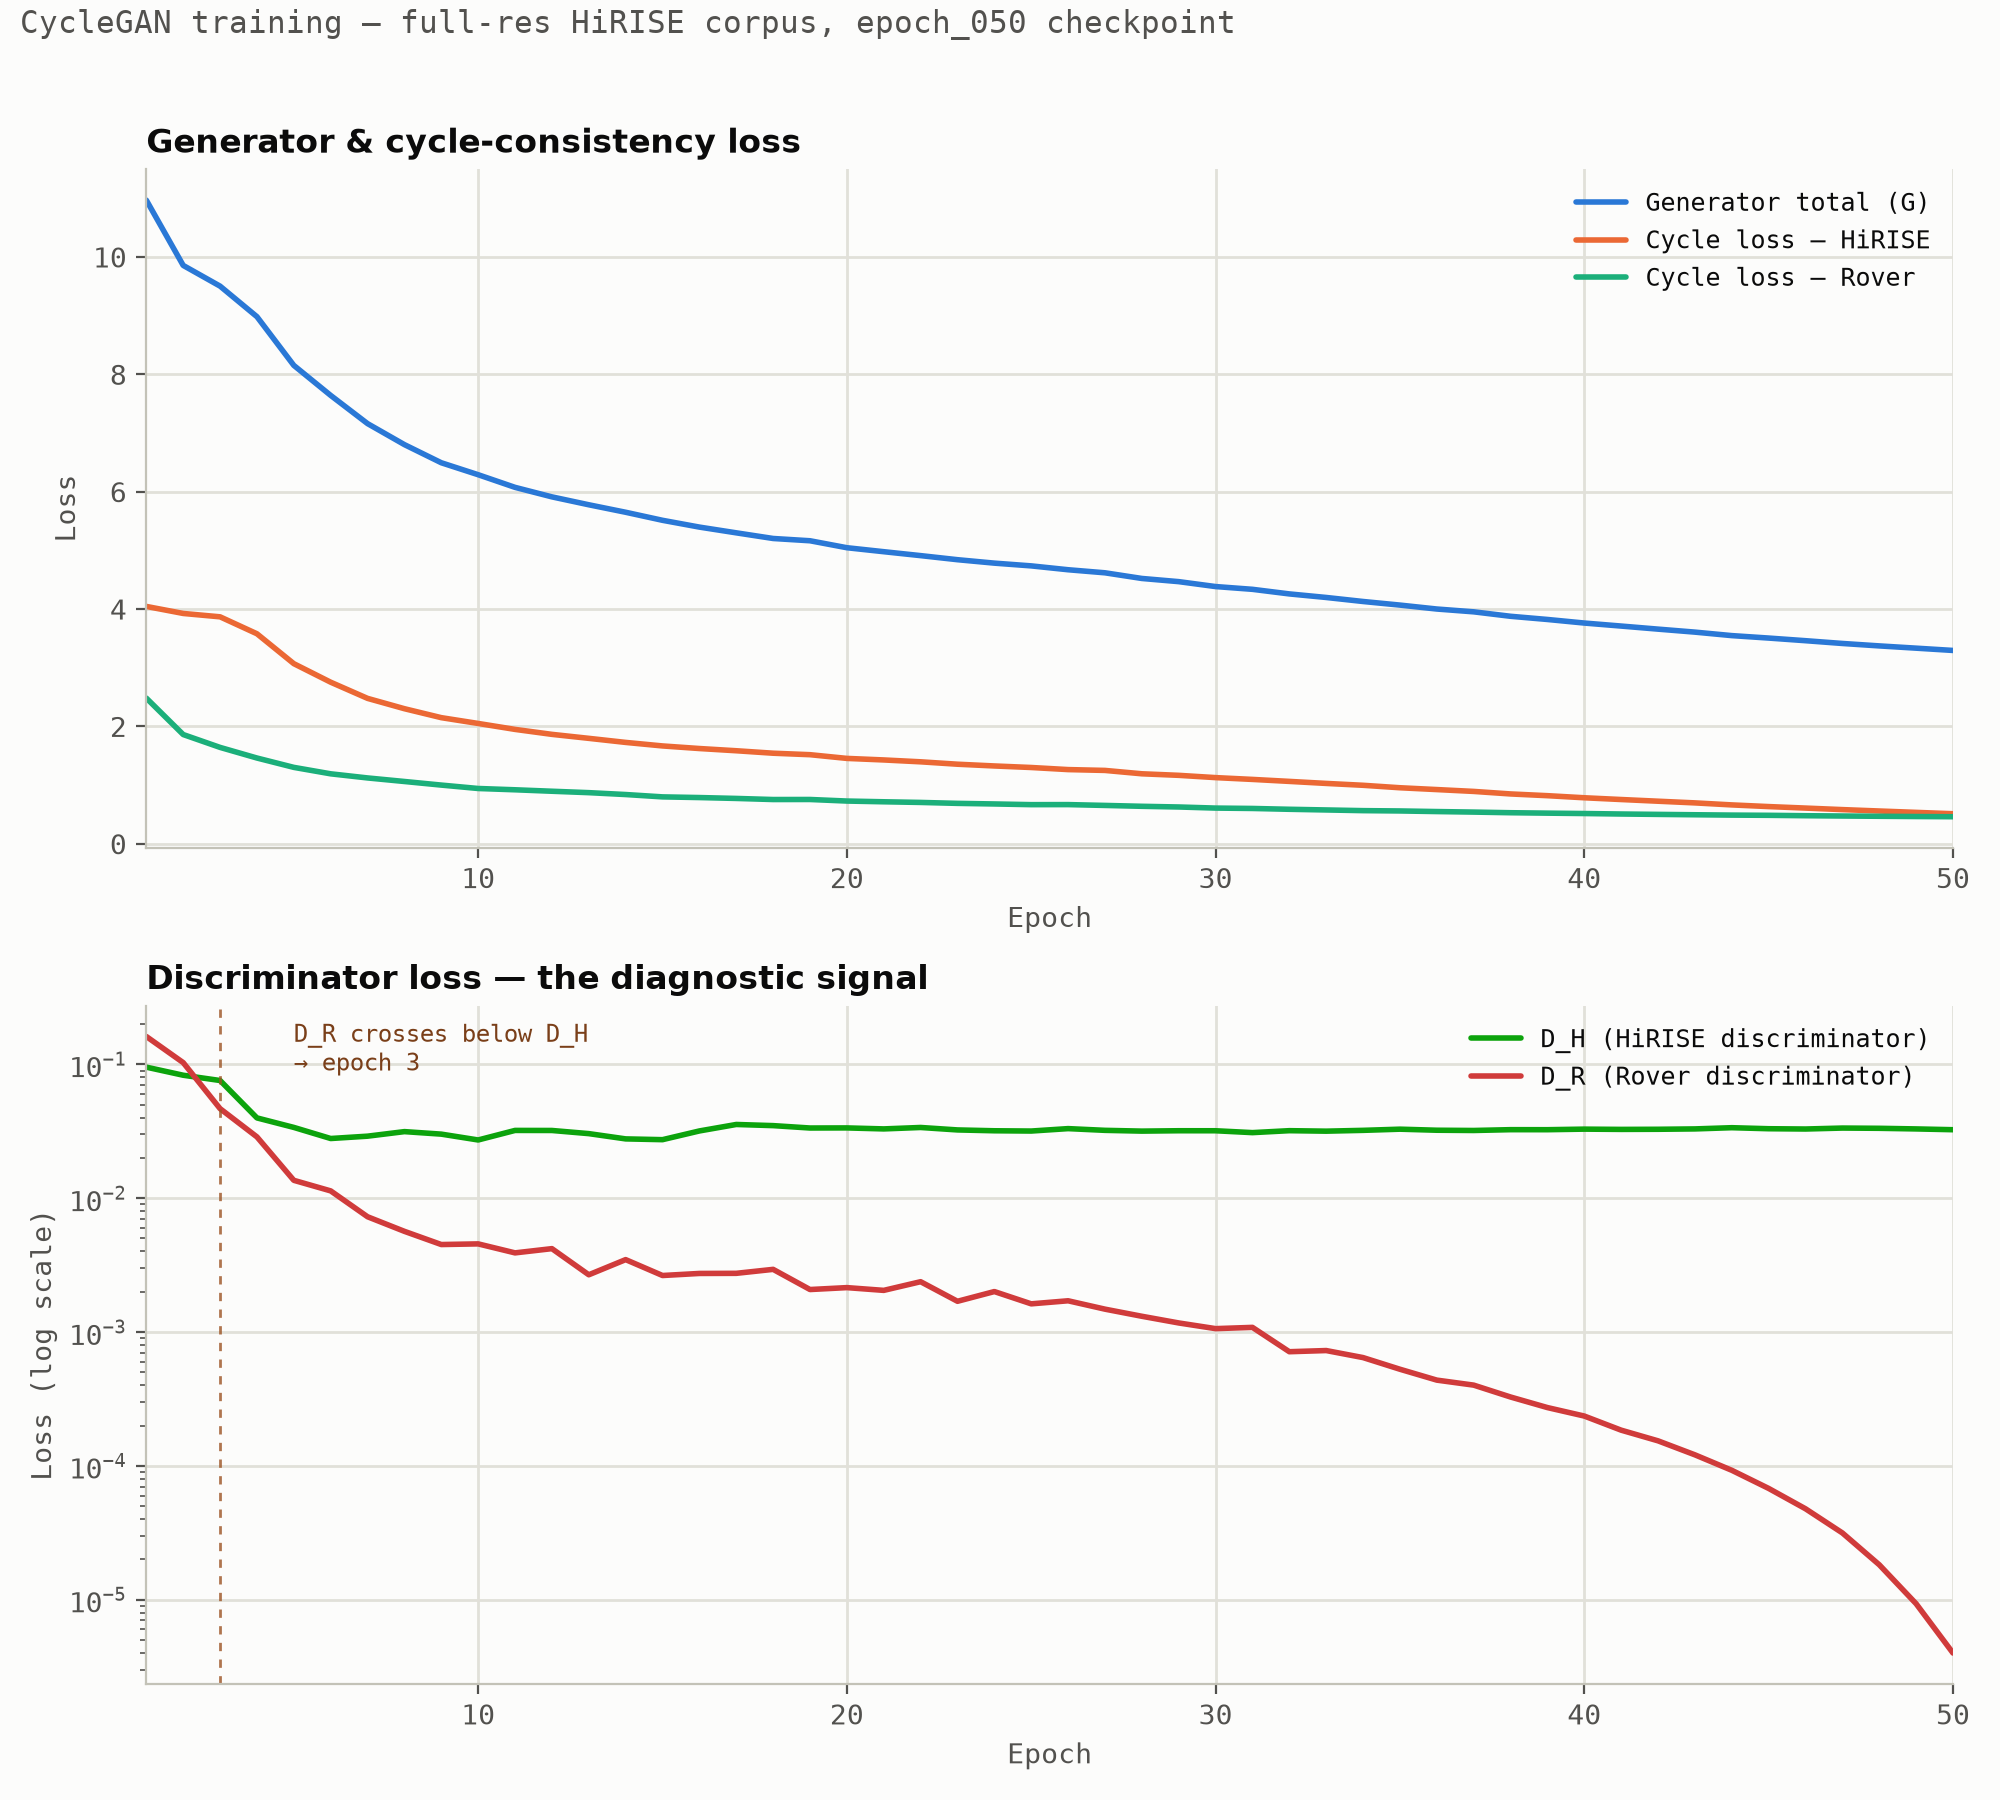
\includegraphics[width=0.95\textwidth]{loss_curves_epoch050}
  \caption{Generator/cycle-consistency loss (top, linear scale) and discriminator loss (bottom, log scale) over 50 epochs of training on the corrected full-resolution HiRISE corpus. $D_R$ collapses from epoch~3 onward while $D_H$ remains stable.}
  \label{fig:losscurves}
\end{figure}

\begin{table}[H]
  \caption{Discriminator loss at representative epochs, illustrating the $D_H$/$D_R$ divergence.}
  \label{tab:disc-timeline}
  \centering
  \begin{tabular}{lrr}
    \toprule
    Epoch & $D_H$ & $D_R$ \\
    \midrule
    1  & 0.0954 & 0.1617 \\
    3  & 0.0758 & 0.0467 \\
    10 & 0.0272 & 0.0046 \\
    25 & 0.0318 & 0.0016 \\
    50 & 0.0325 & 0.0000040 \\
    \bottomrule
  \end{tabular}
\end{table}

\begin{table}[H]
  \caption{FID results against the methodology's target ($\leq$55, Chapter~3).}
  \label{tab:fid-results}
  \centering
  \begin{tabular}{lrrr}
    \toprule
    Run & Checkpoint & Corpus & FID \\
    \midrule
    Prior run  & epoch\_025 & Browse-resolution ($\sim$3\,m/px, buggy) & 171.8 \\
    This run   & epoch\_050 & Real RDR (25\,cm/px, 1 region, 7 obs.) & 269.9 \\
    \midrule
    Target (Chapter~3) & --- & --- & $\leq$55 \\
    \bottomrule
  \end{tabular}
\end{table}

Sample translation grids saved during training (Figures~\ref{fig:sample001}--\ref{fig:sample050}) confirm the same pattern at every epoch inspected: the HiRISE-to-rover translation stays a grainy, high-frequency echo of the input with no rover-ground structure, and both cycle-consistency reconstructions match their originals closely --- a symptom of the underlying problem, not evidence against it.

\begin{figure}[H]
  \centering
  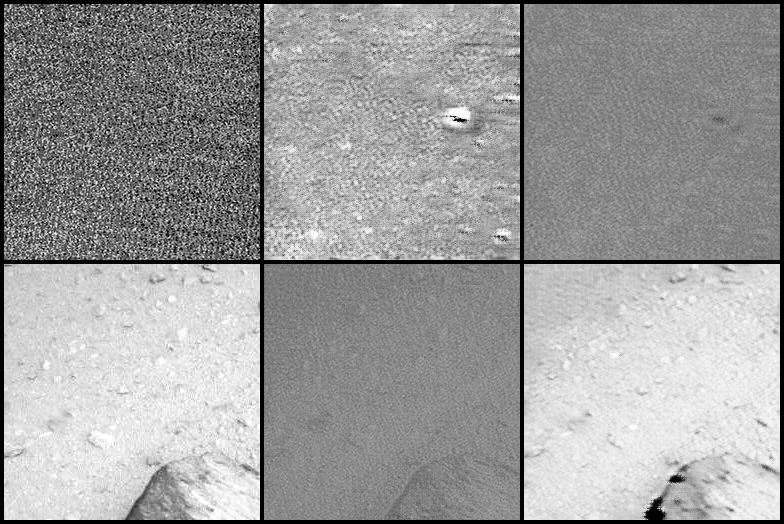
\includegraphics[width=0.75\textwidth]{sample_epoch001}
  \caption{Sample translation grid, epoch 1.}
  \label{fig:sample001}
\end{figure}
\begin{figure}[H]
  \centering
  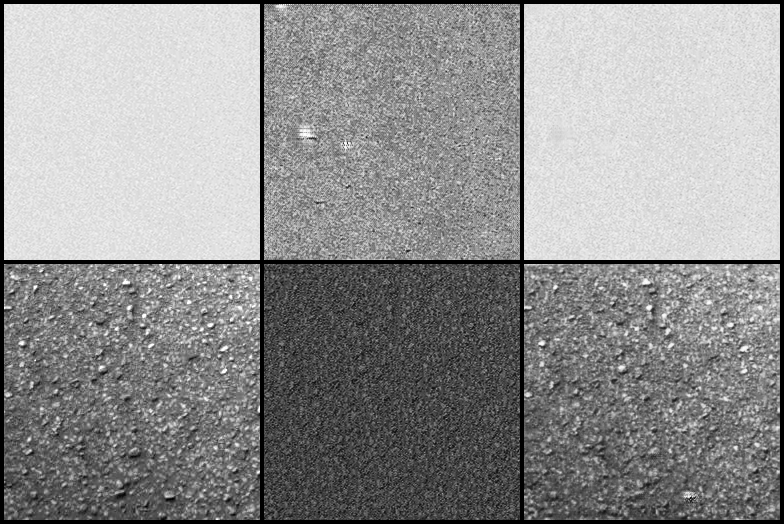
\includegraphics[width=0.75\textwidth]{sample_epoch030}
  \caption{Sample translation grid, epoch 30. $D_R$ is already near collapse (loss $\approx0.0011$).}
  \label{fig:sample030}
\end{figure}
\begin{figure}[H]
  \centering
  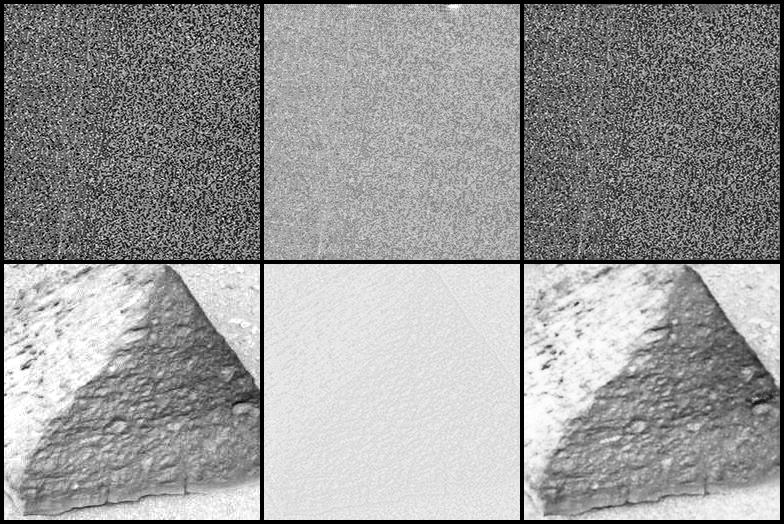
\includegraphics[width=0.75\textwidth]{sample_epoch050}
  \caption{Sample translation grid, final epoch 50 checkpoint.}
  \label{fig:sample050}
\end{figure}

The immediate, epoch-level mechanism is a discriminator shortcut: $D_H$ can reject $G_{H2R}$'s output purely because it still carries the corrected corpus's genuine sensor grain, without needing to learn what a real rover photograph actually looks like, so $G_{H2R}$ receives a real but semantically uninformative gradient once $D_R$ locks onto that shortcut by epoch~3. This also explains why correcting the corpus resolution made FID \emph{worse} rather than better (Table~\ref{tab:fid-results}): the browse-resolution corpus was smoother and closer to rover-image smoothness, so it did not hand $D_R$ this shortcut as blatantly.

\section{A Deeper Root Cause: Corpus Diversity}
\label{sec:diagnosis}

The discriminator-shortcut mechanism above is real, but it is not the whole explanation, and treating it as such would have pointed at the wrong fix. An audit of the corpus that produced the 269.9 result found that of the ten Oxia Planum HiRISE observations the real-resolution pipeline targeted, only seven were available as real, single-band RED JP2 products, and all seven happened to fall in the same region --- collapsing the training corpus from the original browse-resolution pipeline's 299 observations across 4 regions down to 7 observations in 1. Separately, Oxia Planum was deliberately selected as the ExoMars landing site \emph{because} it is smooth and low-relief, while the rover-domain training data (Curiosity, Gale Crater) is comparatively rocky --- a genuine content mismatch layered on top of the diversity collapse, and one that is somewhat inherent to the problem, since no ground-truth Oxia Planum rover imagery can exist before a rover has actually landed there.

A literature review conducted in response to this finding (surveying the super-resolution, image-to-image translation, and cross-view synthesis literature) surfaced a pattern absent from the original three-stage design: published work translating nadir/orbital imagery into ground-level/perspective imagery does not attempt pure pixel-space translation. It inserts an explicit geometric intermediate --- a height field or DTM --- between the nadir input and the perspective output, and synthesises texture only in the already-correctly-projected view. Sections~\ref{sec:track1}--\ref{sec:e2e-results} report two lines of work that followed from this: a loss-tuned CycleGAN retrain that isolates the discriminator-shortcut question from the corpus-diversity question (Track~1), and the geometry-mediated redesign itself (Track~2 onward), built as described in Chapter~4, Section~\ref{sec:geometry-impl}.

\section{Track 1: Isolating the Loss-Weight Question}
\label{sec:track1}

Reducing $\lambda_{\mathrm{cyc}}$ was one of three candidate fixes the original diagnosis proposed for the discriminator shortcut. Testing it cleanly required a corpus that was not itself confounded by the diversity collapse just diagnosed, so Track~1 deliberately trained on the \emph{original}, browse-resolution corpus (37{,}054/4{,}631/4{,}633 HiRISE patches across the full 4 regions, paired with 20{,}417/2{,}552/2{,}553 rover patches) rather than the smaller, single-region real-resolution one --- a resolution/diversity trade-off made explicitly to isolate one variable at a time, and a genuine caveat on how directly Track~1's FID compares against the target, which specifies the true 25\,cm/pixel product.

A 15-epoch, 3-way smoke test on this corpus confirmed the hypothesis: $\lambda_{\mathrm{cyc}}=10$ reproduced the near-identity shortcut, $\lambda_{\mathrm{cyc}}=1$ broke it but visibly degraded output fidelity, and $\lambda_{\mathrm{cyc}}=3$ (paired with $\lambda_{\mathrm{idt}}=1.5$) broke the shortcut cleanly without that degradation. A full 100-epoch run at these validated weights followed (Table~\ref{tab:track1-fid}), with no collapse signature at any point ($D_R$ never approached the earlier run's $10^{-6}$ range).

\begin{table}[H]
  \caption{Track 1 (loss-tuned) FID trajectory, full 4{,}633-image test set.}
  \label{tab:track1-fid}
  \centering
  \begin{tabular}{rr}
    \toprule
    Epoch & FID \\
    \midrule
    15  & 115.73 \\
    25  & 107.54 \\
    35  & 100.53 \\
    45  & 104.45 \\
    55  & 102.62 \\
    100 & \textbf{95.831} \\
    \bottomrule
  \end{tabular}
\end{table}

The run plateaus around FID~100--105 from epoch~35 onward, with the final checkpoint's 95.831 --- Track~1's best, and this dissertation's best CycleGAN FID to date --- only becoming visible once the full 100 epochs completed; the flat loss curves in the learning-rate decay tail apparently still hid a small real improvement.\footnote{\texttt{epoch\_095.pt}'s FID was never computed, having been deleted in a disk-pruning pass before it could be measured; \texttt{epoch\_100}'s 95.831 stands in as the closest available reading, since the run was in a flat loss plateau from epoch~55 through 100.} This is a real fix for the diagnosed shortcut, and a genuine improvement over both the buggy browse-resolution baseline (171.8) and the corrected-but-collapsed corpus (269.9). It is still 1.7$\times$ above the target of $\leq$55, and, more importantly, visual inspection of Track~1's translated outputs at every checkpoint shows the same 2D spatial layout as the input at every epoch --- the crater, stripe, and slope positions do not change. This is not a loss-weight problem: a 2D convolutional generator trained under cycle-consistency has no mechanism to reinterpret scene content from a genuinely different physical vantage point, only to restyle it in place. Only an explicit geometric stage --- Track~2 onward --- can deliver real viewpoint translation, which is the more fundamental reason a pure loss-weight fix cannot reach the target FID on its own.

\section{Track 2: Geometry-Mediated Retraining}
\label{sec:track2}

Track~2 retrains the same architecture and validated loss weights ($\lambda_{\mathrm{cyc}}=3$, $\lambda_{\mathrm{idt}}=1.5$) on the geometry-mediated corpus of Chapter~4 (Section~\ref{sec:geocorpus-impl}): 1{,}513 rendered ground-view images (1{,}210/151/152 train/val/test) from 8 real stereo DTMs in the Oxia Planum landing region, in place of a raw HiRISE crop as CycleGAN's domain-A input. 25 epochs completed with no collapse at any point ($D_R$ stayed in a healthy 0.03--0.5 range throughout).

FID against the real rover test set was 426.0 --- much worse than Track~1's 95.8, but not a fair comparison: the geometry corpus's 152-image test set is small and visually homogeneous relative to the 2{,}553-image real rover distribution, and FID was never really the point of this track. Visual inspection was. It confirms geometry-mediation breaks the near-identity shortcut in a way loss-tuning alone (Track~1) cannot: the previously black, unrendered ``sky'' region above the horizon gets filled with invented texture in the output, and the ground pattern changes structurally rather than merely shifting colour or contrast --- the generator is not just copying its input. But output diversity is compressed: three translations from visually distinct inputs (different horizon shapes) share a dominant chevron/zigzag texture motif. Quantified, the ground-region mean pixel difference between outputs (22--28, 0--255 scale) is lower than between their corresponding inputs (29--40) --- the generator partially, but not fully, tracks input content, leaning on a shared learned texture template consistent with the corpus's own known risk: only 8 distinct source terrains behind 1{,}210 training images.

Geometry-mediation is therefore validated as fixing the specific failure mode that broke Tracks~1 and the original run (the architectural inability to translate viewpoint, and the discriminator shortcut respectively), which is a real, positive result for this dissertation's core methodological claim. But the small corpus caps texture diversity in its current form, and Track~2 does not yet produce convincingly varied rover-eye renders on its own — motivating the separate, paired-supervision texture-synthesis stage (Track~3, Section~\ref{sec:e2e-results}) rather than asking the geometry-mediated CycleGAN to solve texture diversity unaided.

\section{Single-Image DTM Estimation}
\label{sec:dtm-results}

Track~2's renderer needs a real stereo DTM, and only 8 such products exist for the whole landing region. The single-image DTM estimator of Chapter~4 (Section~\ref{sec:dtmestimator-impl}) is evaluated against 21 held-out real Gale Crater patches with a genuine stereo DTM ground truth, achieving a mean RMSE of \textbf{2.02\,m} (std.\ 0.83\,m). Qualitatively, rendering the estimator's own output reproduces the same large-scale artefacts a real DTM's render shows at this site, rather than introducing new ones, and it smooths over the real DTM's stereo-interpolation facet noise while tracking coarse structure --- an expected and acceptable behaviour for a network predicting a physically smooth quantity.

\section{End-to-End Chain: Does the Estimator's Error Actually Matter?}
\label{sec:e2e-results}

The estimator's RMSE is only useful as a number if it can be connected to what actually reaches a viewer: does swapping the real DTM for the estimator's output visibly change the final, texture-synthesised image relative to using ground truth? Answering this required chaining all three geometry-mediation components together for the first time (\texttt{run\_end\_to\_end\_pipeline.py}, Chapter~4 Section~\ref{sec:e2e-impl}) on the same real Gale HiRISE crop, once against the real stereo DTM and once against the estimator's output, both fed through the same Track~3 ControlNet.

The first two attempts were inconclusive. Run at the corpus's default crop location (the raster centre) and a steep $-15^{\circ}$ camera pitch, both the real-DTM and estimated-DTM crude renders stayed dominated by a large, flat, low-texture region --- a ``shelf'' artefact --- leaving neither condition map with much real geometric signal to propagate. A follow-up run at a shallower $-5^{\circ}$ pitch, on the assumption that a steep down-look was responsible, produced the same result: the shelf persisted regardless of pitch, ruling out camera angle as the cause.

A diagnostic tool (\texttt{find\_e2e\_crop\_candidate.py}) built to investigate scored candidate camera positions across the full DTM by \texttt{ground\_entropy} (the same metric used to filter the geometry corpus, Chapter~4 Section~\ref{sec:geocorpus-impl}), and revealed the actual problem: the default crop's render was only 10\% sky, yet scored a low ground\_entropy of 1.92 --- the ``shelf'' is a large, flat, textureless region of \emph{drawn ground}, not an empty frame, which is exactly why changing pitch never helped. Scanning 150 candidate positions found one scoring 6.08, over 3$\times$ higher, at row 6{,}439/column 2{,}730 of the same DTM.

Re-running the full chain at this location, at the original $-15^{\circ}$ pitch, produced the first clean result (Figure~\ref{fig:e2e-newcrop}). The real-DTM and estimated-DTM crude renders now visibly differ in horizon and slope shape (Figure~\ref{fig:e2e-crude-renders}) rather than both being near-blank, and that difference propagates through the Track~3 ControlNet to genuinely different final images: the real-DTM chain's output shows a large dune/rock formation dominating the foreground with strong cast shadows, while the estimated-DTM chain's output shows a flatter rocky plain with different scene framing entirely. This is the first evidence in the project that the DTM estimator's $\sim$2\,m RMSE visibly affects the pipeline's final output, rather than both chains simply converging on the same texture-synthesis prior because the condition signal was too degenerate to carry any real difference.

\begin{figure}[H]
  \centering
  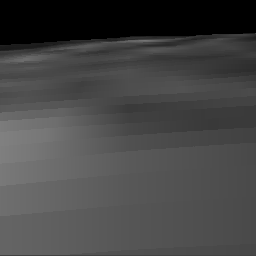
\includegraphics[width=0.48\textwidth]{e2e_newcrop_real_render}\hfill
  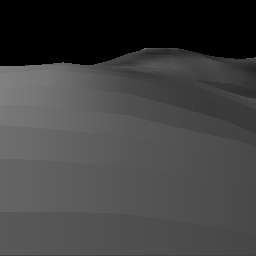
\includegraphics[width=0.48\textwidth]{e2e_newcrop_estimated_render}
  \caption{Crude perspective renders at the high-structure crop, $-15^{\circ}$ pitch: real stereo DTM (left) vs.\ the DTM estimator's own output (right). Unlike every prior test crop, the two now visibly diverge in horizon and slope shape.}
  \label{fig:e2e-crude-renders}
\end{figure}

\begin{figure}[H]
  \centering
  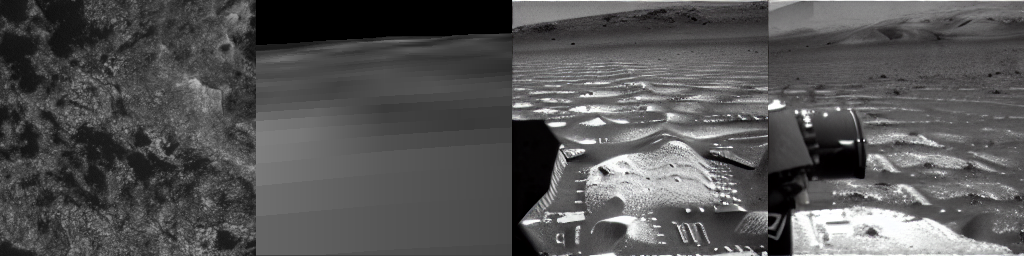
\includegraphics[width=\textwidth]{e2e_newcrop_comparison}
  \caption{End-to-end chain at the high-structure crop, left to right: HiRISE ortho input, real-DTM crude render, real-DTM chain's final Track~3 output, estimated-DTM chain's final Track~3 output. The two final panels diverge in composition, not just texture.}
  \label{fig:e2e-newcrop}
\end{figure}

A caveat carries over from Track~3's own limited corpus: both final outputs still show a repeating ripple/dune texture bias relative to a real (loosely, not camera-matched) reference NAVCAM photo at the same site, which shows far more fine rock-clutter chaos. This is consistent with Track~3's training corpus (27 real paired condition/target images) being small, and is a separate, already-understood limitation rather than a new finding from this test.

\section{Synthesis}
\label{sec:synthesis}

Read against Objective~O2 (Section~1.2), this chapter reports genuine progress and genuine open gaps in roughly equal measure. On the positive side: the original failure was traced to a specific, evidenced mechanism at two levels (a discriminator shortcut, and the corpus diversity collapse behind it), the loss-weight fix for the first was validated in isolation (Track~1), geometry-mediation was validated as fixing the second in the way loss-tuning cannot (Track~2), and today's high-structure-crop test is the first real evidence that the geometry-mediated chain's weakest link --- the single-image DTM estimator standing in for a real stereo DTM --- actually matters to what a viewer would see, rather than being masked by an uninformative test.

On the open side: FID remains 1.7$\times$ above target even at Track~1's best; Track~2's output diversity is compressed by its small, 8-terrain corpus; Track~3's texture synthesis is trained on only 27 real pairs and shows a corresponding texture bias; and the architecture that produced these results --- CycleGAN for viewpoint-preserving restyling, a deterministic renderer for geometry, and a separately-trained ControlNet for texture --- is a different family from the physics-constrained Neural Schr\"{o}dinger Bridge Chapter~3 specifies. Chapter~6 addresses each of these as concrete next steps, including how this last, architectural divergence from the approved methodology should be reconciled.

\chapter{Future Plan}
\label{ch:futureplan}

This chapter sets out the work remaining to complete the dissertation, in the order it is planned to be carried out, and how each item connects back to the objectives in Section~1.2.

\section{Resolve the CycleGAN Discriminator Imbalance}

The most immediate task is acting on the diagnosis in Chapter~5: closing the noise-statistics gap between the real-resolution HiRISE corpus and the rover corpus (most likely via mild denoising of HiRISE patches, matched synthetic grain on the rover side, or both), then retraining and re-evaluating against the same FID and visual-inspection protocol used in Chapter~5. If the diagnosis is correct, FID should drop substantially and the sample-grid translations should stop showing the near-identity mapping documented in Section~5.3. This closes out the CycleGAN baseline for Objective~O2 and establishes the well-understood point of comparison the physics-constrained UNSB is meant to improve on.

\section{Complete the Stage 1 Super-Resolution Corpus}

In parallel with the CycleGAN work, a CTX/HiRISE co-registration pipeline for Objective~O1 is under development: a HiRISE footprint index parser, a Murray Lab CTX mosaic resolver, an orchestration script that produces paired low-/high-resolution crops, and a visual QA tool. A five-image smoke test has succeeded with all pairs correctly aligned; the next steps are a visual confirmation of those five preview pairs, followed by the full batch run across the intended observation set, before any Stage~1 model training begins.

\section{Implement the Physics-Constrained UNSB (Objective O2)}

Once the CycleGAN baseline is resolved, the Neural Schr\"{o}dinger Bridge architecture and the four physics-informed loss terms specified in Chapter~3 (Section~3.1) will be implemented: the shadow-direction, Hapke photometric, and geological morphometry auxiliary networks must each be trained separately before the main IPFP training loop (Algorithm~\ref{alg:stage2}) can run. This is the central remaining engineering task and the dissertation's core methodological contribution. The CycleGAN results in Chapter~5 already provide a concrete, measured baseline (FID, and the specific discriminator-imbalance failure mode) that the physics-constrained architecture will be evaluated against, rather than only against literature-derived estimates.

\section{Gaussian Splatting Rendering (Objective O3)}

Once Stage~2 produces usable synthetic perspective imagery, a 3D Gaussian Splatting scene will be trained on the resulting multi-view set, following the reference implementation and the MADNet-2.0-seeded initialisation described in Chapter~3, and benchmarked for render throughput against the $\geq$72\,fps VR target.

\section{Full Evaluation (Objective O4)}

The evaluation framework in Chapter~3 (Section~3.4) --- FID and LPIPS, structural fidelity against synthetic ground truth, shadow-angle error, Hapke BRDF residual, hallucination rate, and VR render quality --- will be applied to the completed pipeline and compared against the four baselines in Table~\ref{tab:baselines}, including the CycleGAN baseline now measured directly (Chapter~5) rather than estimated from the literature.

\section{Indicative Timeline}

Resolving the CycleGAN diagnosis and completing the Stage~1 co-registration batch are the near-term priorities, since both feed directly into Stage~2 training. UNSB implementation and training is the largest remaining task and is expected to require the majority of the time before the next milestone. Gaussian Splatting integration and the full evaluation pass follow once Stage~2 produces synthetic imagery of sufficient quality, with time reserved at the end for writing the Results/Evaluation and Conclusions chapters that this draft does not yet include.



%%%%%%%%%%%%%%%%%%%ETC%%%%%%%%%%%%%%%%%%%%%%
\addcontentsline{toc}{chapter}{Bibliography}
\bibliographystyle{./style/myabbrvnat}
\bibliography{./references/thesisbib}

\end{document}
